\section{Title}\label{title}

Towards a metabolic theory of island biogeography

\section{Abstract}\label{abstract}

Food webs structure the partitioning of energy from the primary
producers to the top predators. Although energy is one of the most
important factor diversity, it remains overlooked by classical theories
in biogepgraphy that either assume ecological equivalence (\emph{e.g}
the TIB) or remain focused on the concept of the ecological niche.
Energy is however a factor early envisioned as a key to understand the
structure of food web and the coexistence of species. Classical
gradients in biogeography are linked to energy such as latitudinal
diversity gradient. Moreover the classical view of biomes is actually
rooted on energy and water availibities. Therefore funding a theory of
biogeography on the bases a energy partitioning among food is a
promising avenur to gather diffenret pece of infornation within one
conceptual framework. Here we undertake such integrated model that
integrate energy contrain as quantity of primary producers on the island
and take different into account. We derive an assemblage nased on
stochastic colonisatin and randonm. Bases on we show how energy
consriant the food web and how enegry transfer efficiency is important.
l'impact des interactions trophiques sur la distribution de la
biodiversité au long de gradients de productivit. along gradient As a
consequence, our theory encompasses both the species-area and the
species-energy relationships, making it a very general framework to
understand and predict biodiversity distribution

\section{Introduction}\label{introduction}

Disentangling the relative contribution of the different processes
shaping biodiversity distribution is the central objective of
biogeography. While biogeographers clearly envision the list of
ingredients needed to understand species distribution
\citep{Thuiller2013}, they miss the framework to mix them in the right
amount and to investigate the biogeography of ecological communities. We
will likely fail to predict accurately biodiversity responses to global
changes as we keep our focus strictly on abiotic factors \emph{i.e}
temperature and precipitation, while continuing to overlook biotic
interactions \citep{Wiens2011} and short-term evolutionary responses
\citep{Lavergne2010}. At the core of this issue is the need for an
integrated approach at the crossroad between species distribution
modelling and community ecology.

Biotic interactions should be integrated as a constraint for species
co-distribution in meta-communities \citep{Jabot2012, Cazelles2016a}.
Ecological interactions may explain, at least partially, the dynamics of
local extinctions, which in turn would further explain some properties
of the geometrical shape of species ranges \citep[\emph{e.g.} nested
distributions of parasitoid and its host,][]{Shenbrot2007}. We have
however limited evidence of the effect of biotic interactions on large
scale species distribution \citep[see Chapter \ref{chap3} - but
see][]{Gotelli2010}. Incidentally, two of the most influential models in
biogeography assume ecological equivalence of species; the Theory of
Island Biogeography of MacArthur and Wilson \citep[hereafter
TIB,][]{MacArthur1967} overlook the variation among species
characteristics and ignore their arrangement in organized ecological
networks. In his neutral theory, Hubbell assumes that individuals of
different species are ecologically equivalent and predicts the
distribution of abundance without considering interactions
\citep{Hubbell1997, Hubbell2001}. These two theoretical models have been
proven relevant for certain groups of species and inadequate for others,
and none of them were initially intended to describe exhaustively the
structure of ecological communities. The integration of ecological
interactions into biogeography however offers promising perspectives and
a much extended range of predictions \citep{Holt2010, Gravel2011}.

The TIB is well-suited to explore the consequences of ecological
interactions on community structure at broad spatial scales, as it
includes two fundamental processes of biogeography, immigration and
extinction, in an elegant fashion that eases its extension
\citep{Losos2010, Warren2015}. Building upon the classical model of
MacArthur and Wilson, recent studies have included various forms of
interactions in the TIB \citep{Gravel2011, Cazelles2016a}. The regional
species pool becomes a \emph{metaweb}, not only listing potential
colonists but also their interactions. With this approach, species are
inter-dependent entities with specificities (\emph{e.g.} a given trophic
level) rather than indistinguishable units. As a consequence,
colonization and extinction rates vary with respect to species identity
\emph{and} the composition of the local community. \citet{Gravel2011}
proposed the Trophic TIB (hereinafter TTIB) to represent food web
assembly on isolated communities, where predators can persist locally as
long as they find at least one preys. More generally,
\citet{Cazelles2016a} presented a Lotka-Volterra like model in which the
composition of the local community determines both colonization and
extinction rates. Adding new ecological processes in the TIB increases
realism, at the cost however of reducing its simplicity. It provides an
extended list of predictions, which have yet to be proven significantly
better than the original theory \citep[see][]{Cirtwill2015}. Extending
the TIB while preserving its elegance is a challenging and technical
issue. Here we propose to reformulate the TTIB in terms of energy
constrains in attempt to solve this challenge.

The TIB was originally meant to predict and explain the common
observation of increasing species richness with island area. Another
ubiquitous and fundamental observation in biogeography is the
latitudinal diversity gradient
\citep[LDG,][]{Rhode1992, Stevens1989, Evans2005}. The productivity of
primary producers is generally found the best predictor of species
richness at large spatial scales \citep{Evans2005, Storch2005}. Others
found a strong correlation between richness, water availability and
temperature \citep{Currie1993, Hawkins2003}. Several mechanisms have
been proposed to explain this relationship \citep[see][ for a
review]{Currie2004, Evans2005}, including higher speciation rates in
tropical areas, greater biomass and finer niche partitioning. Recently,
some authors investigated how networks could change with latitude. Based
on the meta-analysis of 196 empirical food webs, \citet{Cirtwill2015a}
shown that ecological networks of interactions also vary along this
gradient but that the density of links remains constant throughout. In
the majority of ecosystems theses authors studied, an increased energy
results in a wider niche space, rather than an increase of niche breadth
poleward. Similarly, \citet{Albouy2016} reconstructed marine networks
across the globe and found significant latitudinal-network gradients
(LNG). These studies are however descriptive only, as there is currently
no theory to explain how and why energy constraints should impact food
web structure. In 1983, \citet{Wright1983} developed the species-energy
theory and replaced the ``area'' with ``available energy'' to derive a
meaningful Species Energy Relationship (SER). Although area and energy
may bring more information taken together \citep{Storch2005}, the
rationale behind it allows the derivation of species abundance and
occurrence probability based on energetic constraint \citep{Wright1983}.
Wright's approach however do not specifically account for network
structure and thereby remains limited to species richness.

Species do not escape from the laws of thermodynamics and as a
consequence, despite the complexity of evolutionary trajectories, many
key ecological properties and processes scale with body mass
\citep[\emph{i.e.} metabolic theory of
ecology][]{Brown2004, Woodward2005a}. The scaling of the metabolic rates
with body mass is the fundamental observation underlying this theory
\citep{Gillooly2001}, which typically follows a power function with
coefficients often between 2/3 and 3/4 \citep{White2013}. Even if all
the relationships are not well-understood \citep[see the case of
abundances reviewed in][ and the recent relationship between prey and
predator biomasses \citet{Hatton2015}]{White2007}, the ubiquity of
allometric relationships makes body mass distribution a key variable to
reduce the complexity of ecosystems. Allometric relationships and energy
flows also provide the mean to parameterize models of population
dynamics \citep{Yodzis1992}. Recent developments of food web theory have
convincingly shown that allometric relationships are the cog to analyze
the properties of ecological networks \citep{Gravel2013, Petchey2008},
their dynamics \citep{Brose2006} and to characterize the role of species
within them \citep{Schneider2012}.

Our objective in this study is to develop a theory of biodiversity
distribution based on first principles of energetic constraints in order
to investigate the impact of trophic interactions on the
latitudinal-diversity gradient. We propose to extend the model of the
TTIB following the vision of \citet{Wright1983}. As a consequence, our
theory encompasses both the species-area and the species-energy
relationships, making it a very general framework to understand and
predict biodiversity distribution. In addition, the explicit integration
of trophic interactions allows the development of a vast array of
testable and insightful predictions, including the expected
latitudinal-network gradient. To do so, we propose a theoretical model
of food web assembly driven by colonization from the regional metaweb
and energetic constraints. We derive expected species richness and
network structure along gradients of primary productivity. We use
``Lindeman'' \citep{Lindeman1942} transfer efficiency (\emph{i.e.}
energy transferred to another trophic level) to integrate
species-specific differences in their source of energy. We derive a SER
and the relationship between body-mass distribution and available
energy. Our model formalizes the initial hypothesis of Lindeman and
offers immense possibilities for the integration of community ecology
with biogeography.

\section{Model description}\label{model-description}

The model developed by MacArthur and Wilson predicts species richness on
an island according to the size of the island and its distance from the
mainland \citep{MacArthur1967}. One promising direction to extend this
theory is to include biotic interactions into the classical model
\citep{Holt2010, Gravel2011, Cazelles2016a}. Following this avenue, we
consider explicit interactions among the regional pool of species based
on allometric relationships. Body mass is used to determine the quantity
of energy a given species requires to maintain its local population on
an island. Extinction follows if the island cannot sustain a minimal
population of any given species. Therefore, in the model described
below, we simulate the TIB with purely stochastic colonization events
together with deterministic extinction based on an energy rational.

We consider an island as an isolated piece of land covered by a maximal
quantity of primary producers, which determine the amount of available
energy upon which a food web can develop. We denote \(E_0\) the maximal
amount of energy available for herbivores and consider it to vary
proportionally to island area. Here we do not enter the specificities of
how productivity scales with area, as in some situation it could scale
linearly or not (e.g.~for lakes when the volume determines productivity,
Post et al. 2000). As a consequence, the model explains both the scaling
of richness with island area and productivity, with the same underlying
principle that a minimal population size is required for persistence. We
make two additional simplifications: the diversity of primary producers
is not taken into account, and the production is constant over the time.

The regional pool of species in the TIB is the number of species \(P\)
and the tropic interactions among them. Following \citet{Cazelles2016a}
, potential interactions among them are determined using the niche model
\citep{Williams2000}. We furthermore assume the niche axis to be the
body size of the species \citep{Gravel2013} and that species which are
without any links in the metaweb are determined to be herbivores. Note
that primary producers are not included in the niche model but the
source of energy of herbivores. THERE NICHE POSITION IS\ldots{}\ldots{}
As a consequence, trophic level is strongly correlated to body mass,
with herbivores often the smallest and top predators the largest.
Although this assumption is an oversimplification of the determinants of
ecological interactions, it remains reasonable for marine ecosystems
\citep{Trebilco2013}, where allometric relationships have been used to
infer food web structure \citep{Gravel2013}.

Following \citet{Gravel2011}, we assume that the colonization of
herbivores/predators is successful only if they find at least one of
their habitat/prey on the given island. Additionnally, we propose that
colonization events are possible only if the energetic requirements to
maintain local populations exceeds the primary production. In this case,
energetic constraints and network topology determine the identity of
species to go extinct. Colonization events are assumed to be purely
stochastic, while extinctions are more deterministic \citep[this
difference in stochastic nature between these fundamental processes of
biogeography has been recently supported in][]{Cirtwill2015}.

\subsection{Energetic constraints on local food
webs}\label{energetic-constraints-on-local-food-webs}

The rational for energetic constraints is simple: local populations need
a certain amount of energy to maintain a minimum level of activity
otherwise they die from starvation. Under this constraint, species
richness locally increases until the energy production is no longer
sufficient for all populations because of inefficient energy transfer at
each trophic interactions.

We now needs to define a rule to set the the minimal energy a population
needs to survive on the island. For a given species \(i\), energy
requirements of any individual is derived from allometric relationships
proposed by the metabolic theory of ecology \citep{Brown2004}, of the
form \(c_im_i^b\). We do not integrate intraspecific variability in body
mass and thus \(m_i\) is a constant for a species The energy uptake
associated to a minimal viable population (hereafter MVP) of \(n_i\)
individuals becomes \(n_im_i^b\). \citet{Shaffer1981} defined the MVP as
``\emph{{[}\ldots{}{]} the smallest isolated population having a 99\%
chance of remaining extant for 1000 years despite the foreseeable
effects of demographic, environmental and genetic stochasticity, and
natural catastrophe}'', highlighting that the smallest portion of a
population has the highest possible extinction risk (extrapolated as
time to extinction). The key problem is wether or not the MVP is size
dependent. The most conservative assumption is to consider it to be a
constant. \citet{Lande1993} however shown that the time to extinction is
affected by the mean population growth rate, which underlies that
species characteristics may lead to a heterogeneity in MVP. Moreover,
\citet{Savage2004} had developed a framework within which they proved
the growth rate to be proportional to \(m_i^{-b}\). Based on these
results, we explore two different rules for extinctions: (1) MVP is
equal for all species: \(n_i=n_0\), and (2) MVP scales with the growth
rate \(n_i=n_0m_i^{-b}\). For both scenarios, species \(i\) can survive
only if the energy expenditures can be covered, \emph{i.e} if the energy
available is greater than: \(n_ic_im_i^b\).

\subsection{Energy fluxes and transfer
efficiency}\label{energy-fluxes-and-transfer-efficiency}

Although the expression of energy consumption is similar among species,
they obtain it from different sources: herbivores feed on primary
producers, whereas predators feed on a set number of secondary
consumers. The primary production must therefore be tracked as it moves
up through the food chain. To deal with this, we propose to convert the
energy costs for maintaining predator populations into additional
populations of herbivores to be maintained. To exemplify this idea, we
start with the simplest trophic network where a predator \(j\) feeds
upon a herbivore \(i\). The cost to maintain the MVP of \(i\) is
\(n_ic_im_i^b\) and \(n_jc_jm_j^b\) for \(j\). For the latter, we
convert \(n_j\) into an extra population of \(i\), \(n_{i,j}\) herbivore
individuals dedicated to \(j\) consumption. Furthermore, we account for
the energy loss during consumption by including a transfer efficiency
(sensu Lindeman1942) \(\tau\). Hence, the conversion from \(n_{j}\) to
\(n_{i,j}\) is given by the following equation:
\begin{equation} \tau n_{i,j} c_im_i^b = n_jc_jm_j^b \label{eq:id1}\end{equation}

which yields the population size:

\begin{equation} n_{i,j} = \frac{n_jc_j}{\tau c_i} \left( \frac{m_j}{m_i} \right)^b \label{eq:id2}\end{equation}

We postulate that the transfer efficiency is constant across trophic
levels, which is likely an oversimplification of the reality as
suggested by the sparse empirical data available
\citep{Trebilco2013, Brown2003}. We now add a new predator \(k\) feeding
on \(j\) (the predator of \(i\)) to the insular food web. According to
our reasoning, we must covert \(n_k\) into \(n_{i,k}\). To do so, we
start by converting \(n_k\) into a population of \(j\):

\begin{equation} n_{j,k} = \frac{n_kc_k}{\tau c_j} \left( \frac{m_k}{m_j} \right)^b \label{eq:id2}\end{equation}

We now turn \(n_{j,k}\) into a herbivore population:

\begin{equation} n_{i,k} = \frac{\frac{n_kc_k}{\tau c_j} \left( \frac{m_k}{m_j} \right)^bc_j}{\tau c_i} \left( \frac{m_j}{m_i} \right)^b \label{eq:id3}\end{equation}

which gives:

\begin{equation} n_{i,k} = \frac{n_kc_k}{\tau^2 c_i} \left( \frac{m_k}{m_i} \right)^b \label{eq:id3b}\end{equation}

In a similar fashion, for a linear trophic chain, we can demonstrate
that the additional population of herbivore \(i\) necessary to maintain
predator \(j\) of level \(l\) is:

\begin{equation} n_{i,k} = \frac{n_jc_j}{\tau^l c_i} \left( \frac{m_j}{m_i} \right)^b \label{eq:id4}\end{equation}

In many cases, a predator feeds on an array of prey species rather than
a single one. As such, it uptakes its energy from the different sources
and we must account for all of them. We assume that energy costs
associated with maintaining the local predator are minimal. Therefore,
\(n_j\) is converted into \(i\), the herbivore linked to \(j\) for which
(\ref{eq:id4}) is minimal. Basically, \(i\) should be a large and
separated from \(j\) by a low number of species. Hence, on the island,
the species richness increases as long as the inequality below holds
true:

\begin{equation} \sum_i c_in_im_i^b + \sum_j \frac{n_jc_j}{\tau^{l_j} c_i} \left( \frac{m_j}{m_{i_j}} \right)^b < E_0 \label{eq:id5}\end{equation}

The first term is the energy cost for maintaining populations of
herbivores, the second term is associated to higher trophic levels:
predator \(j\) is converted into herbivore \(i_j\) from which it is
separated by \(l_j\) links. For the sake of simplicity, we make an extra
assumptions: \(c_i\) values are constant among species and set to 1.
Therefore, if we assume that MVP is constant (scenario 1), inequality
\ref{eq:id5} becomes:

\begin{equation} \sum_i m_i^b + \sum_j \frac{1}{\tau^{l_j}} \left( \frac{m_j}{m_{i_j}} \right)^b< \frac{E_0}{n_0} \label{eq:id5a}\end{equation}

Similarly, if we assume \(n_i=n_0m_i^{-b}\) and \(n_j=n_0m_j^{-b}\)
(scenario 2), then:

\begin{equation} \sum_i 1 + \sum_j \frac{1}{\tau^{l_j}} \left( \frac{1}{m_{i_j}} \right)^b< \frac{E_0}{n_0} \label{eq:id5b}\end{equation}

The left side of this equation provides the minimal energy needed to
sustain all populations while the right side is the total amount of
energy available. Therefore, the maximal population of species \(i\)
without any extinction is given by converting the extra amount of energy
available into an additional population of species \(i\), the population
of \(i\) we get is denote \(n_{i,max}\). The range \([n_i, n_{i, max}]\)
is then the range of possible fluctuations of species \(i\) without any
new extinction event.

\subsection{Extinctions}\label{extinctions}

When the local primary production cannot sustain the establishment of a
new immigrant, \emph{i.e.} when inequality \ref{eq:id5} is no longer
verified, its arrival is either impossible or lead to extinction of
other species. In the latter situation, we must determine the identity
of species that will go extinct, which remains a significant challenge
that will not be undertaken here given its complexity highlighted by
recent theoretical studies \citep{Saterberg2013, Zhao2016}. To overcome
this concern, we use two scenarios: (1) \emph{random extinction}: any
species can go extinct, and (2) \emph{costs-based extinctions}: the
probability of extinction is proportional to the energetic costs of the
species. Once an extinction occurs, we ensure that all species remain
linked to at least one herbivore, otherwise unlinked species will too go
extinct. Finally, extinctions are set to occur until \ref{eq:id5} is
satisfied.

Although the assumptions we have made here are likely unrealistic, our
intentions are merely to examine the model under the special case of an
optimal energy allocation on an island. These assumptions remain
acceptable as long as we focus on the qualitative consequences in term
of community dynamics. As an important remark, the energy cost
associated to one predator is not based on inherent properties only, as
it is determined also by the identity of its preys present on the island
(in otehr words, via apparent competition). Hypotheses made for the four
scenario are recapitulated in Table \ref{tbl:scena}.

\begin{longtable}[]{@{}lll@{}}
\caption{Hypotheses associated to the four scenarios.
\label{tbl:scena}}\tabularnewline
\toprule
Scenario & MVP & extinction\tabularnewline
\midrule
\endfirsthead
\toprule
Scenario & MVP & extinction\tabularnewline
\midrule
\endhead
A & \(n_0\) & random\tabularnewline
B & \(n_0\) & costs-based\tabularnewline
C & \(n_0m^{-.75}\) & random\tabularnewline
D & \(n_0m^{-.75}\) & costs-based\tabularnewline
\bottomrule
\end{longtable}

\subsection{Simulations}\label{simulations}

Every simulation starts with the generation of the regional metaweb of
100 species. To do so, we first draw a number \(p_i\) for all species
from a uniform distribution from the range {[}0,3{]}. Numbers \(p_i\)
are then sorted, the lowest values are assigned to the herbivores and we
use the vector obtained as the niche axis in the niche model, with
connectance set to \(0.05\) \citep{Williams2000}. Species that are not
connected are assumed to be herbivores and to allow comparisons among
simulation we standardize the number of herbivore to 10. To do so we
keep generating new metawebs until one we obtain one metweb with 10
species that were not connected. We also use the \(p_i\) number to
derive the biomass of all species, we do so by using \(10^{p_i}\). The
smallest species has the smallest niche axis.

We simulated the model along a gradient of energy ranging in
\(\frac{E_0}{n_0}\) from \(.1\) to \(10^8\). We start with an empty
island and at any time step, any species of the metaweb has a
probability \(c=0.001\) of colonizing the island. If a successful
colonization occurs if available energy on the island allow to sustaint
a MVP of the new species. For all time step we record the species on the
island. We perform 125,000 iterations and discard 25,000 burn-in
iterations and the 100,000 remaining to do our analyses. For all the 91
values of the energy gradient we used 100 replicates, meaning 100
different regional metawebs.

\section{Results}\label{results}

We found a sigmoidal SER for all scenarios (Fig. \ref{fig:etib1} A).
Under scenario A, for instance, species richness increased exponentially
with the increase in energy, where more species were allowed to colonize
the island (Fig. \ref{fig:etib1}). SER reached saturation much faster
under scenarios C and D than under the scenarios A and B, due to the
difference in energy uptake. Under scenarios C and D the MVP decreased
with body mass, which allows higher species richness or a comparable
amount of energy. Remarkably, species richness was smaller for scenarios
where the extinction rate was cost-based than randomly based (Fig.
\ref{fig:etib1} A-B), which also results in less variability (Fig.
\ref{fig:etib1} C).

Occurrence probability increases with available energy and decreases
with trophic level for all scenarios (\ref{fig:etib2}). Herbivores were
found to colonize the island first, followed by predators of increasing
trophic level. The trend was similar for all scenarios, and more
pronounced for those where extinction is cost-based (scenarios B and D).
When species occurrence probabilities were grouped by body mass, only
significant differences were found within scenario B (\ref{fig:etib3}).
Taken together, these results highlight the importance of network
structure. Here, we outline the importance of colonization, where the
shortest path between herbivore and predator is extremely important
especially given it strongly impacts the cost of a species; suggesting
that this is the cause of the main differences among random and
cost-based extinction rates.

The average species body mass increased with energy under scenarios A
and B, but decreased under scenarios C and D. The reduction of MVP with
body mass would therefore allow for larger species to maintain on small
island (\ref{fig:etib4} A-D). We see a similar trend for the number of
prey species, which increases with energy in scenarios A and B, while it
decreases in scenarios C and D (\ref{fig:etib4} E-H). Ultimately,
generalist species have a much higher rate of successful colonization
under low energy in scenarios C and D. When the MVP is smaller, larger
species can colonize and their probability of success is higher as they
have more preys in average \citep[due to the use of the niche model and
body mass as the niche axis][]{Williams2000, Gravel2013}. Finally, under
scenarios A and B small species with several predators colonize low
energy islands while under scenarios C and D the same species colonize
the island with higher energy availability as they are preceded by
larger and more generalist species \citep[ I-L]{fig:etib4}.

\section{Discussion}\label{discussion}

We proposed a of the classical TIB in terms of energy and turns the
well-known colonization/extinction dynamics into an successional
assembly process, starting with herbivores and then building up the food
web. We link species extinction to energy requirements, making
extinctions more mechanistic than in the TIB. Moreover, species are no
longer ecologically equivalent as in TIB \citep{Lomolino2009}, they have
a body mass, a trophic level and specific interactions. Based on these
characteristics, we compute a cost associated to the MVP on the island.
Therefore an insular community become an assemblage of population that
should not exceed a given amount of energy. Although the energy
allocation we use here is simple, we think it is a significative step
towards the interactions of community dynamics in biogeography theory.
The next step would be to integrate more realistic energy partitioning
\citep{DeRuiter1995} and taking both bottom up and top-down effects into
account \citep{Terborgh2001, Brown2013}. This remains a real challenge
but also a promising avenue toward a more mechanistic biogeography

Our findings reveal how energy constrains assembly dynamics. Notably,
the linear relationship between the logarithm of species richness and
the log of available energy (\ref{fig:etib1} B) is consistent with
empirical observations (see Fig 3. and Fig 4. in \citet{Wright1983}).
Over evolutionary scales, it would also be consistent with the
Ecological Limits hypothesis to diversification dynamics
\citep{Rabosky2015}. Moreover using the trophic status of species, we
observed a clear relationship between the position in the food webs and
the energy limitations, indicating that food-chain length is limited by
availability energy. A comparable relationship has already been observed
by \citet{Post2000}, who have found a correlation lamong maximal
food-chain length and lake size. Our relationship links food-chain
length and energy available which is partially correlated with area.
Indeed even if area has no direct effect of organism, it actually
correlates with energy but the information could complete each other
\citep{Storch2005}. Hence, the total energy available in the lake could
a better explanation for the relationship theses authors unraveled.
Also, the size of the lake is correlated to the a the habitat
heterogeneity which also influence the diversity of species
\citep{Allouche2012}. Another step forward would be to tease apart the
effect of area, energy and heterogeneity in a model of insular
biogeography. As a possible avenue, we could consider a variably among
primary producers in our model using difference sources of energy to
micmic habitat heterogeneity.

Using our framework, we have shown that under scenarios C and D in which
MVP decreases with the body mass, larger and generalist species are the
first to colonize the island. Remarkably, the early colonization of
generalist species has been highlighted by \citet{Piechnik2008} when
they revisited the classical study by \citet{Simberloff1969}. Also,
reading Fig \ref{fig:etib4} G-H in the direction of a loss of energy,
such as in the case of habitat fragmentation, we observe an increasing
in generalist species such as currently observed \citet{Clavel2011}.
Beyond this observation, the reformulation of TIB in terms of energy we
achieved offers great hope towards a more mechanistic biogeography.
First, energy expressed as a quantity of primary producers per time unit
is readily linkable to climate variables
\citep{Wright1983, Hawkins2003, Evans2005}. Second there is a clear
relationship between physical constrains of the island and the maximal
number of species it can sustain. Third, we used a regional metaweb
which introduces variability among species as well as inter-dependency
among the pool of species \citep{Gravel2011}. Finally, we link all these
using an energy rational grounded on the metabolic theory of ecology
\citep{Brown2004}. We think such achievement provides the first bricks
to pave the avenue towards a metabolic theory of biogeography that could
potentially propose theoretical explanations to the pervasiveness of
surprising allometric scaling poorly understood \citep{Hatton2015}.

\begin{figure}[htbp]
\centering
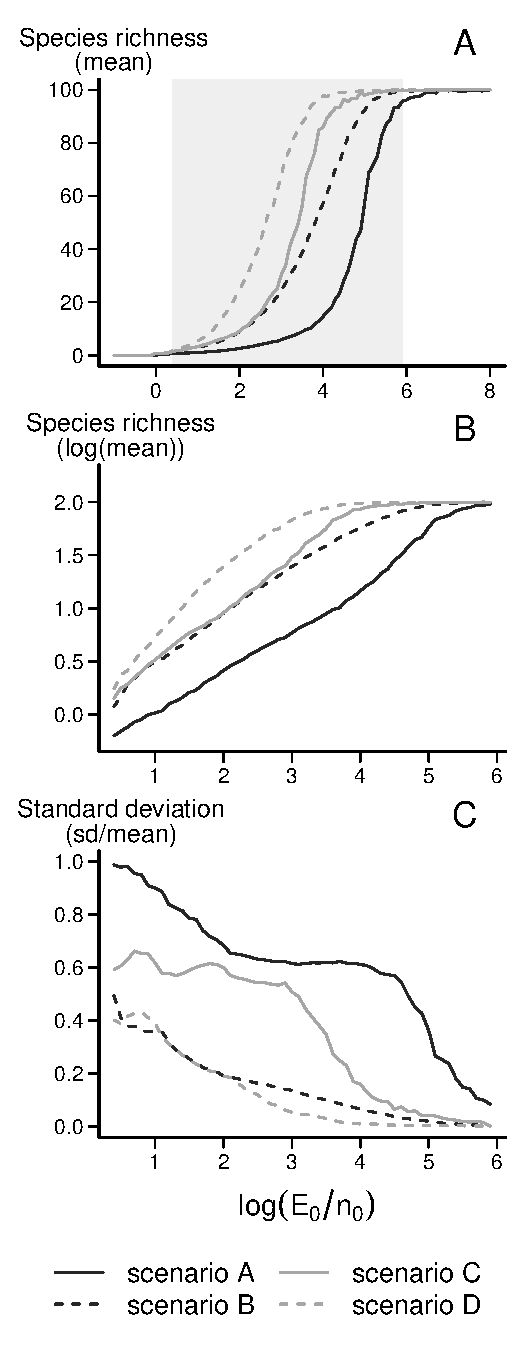
\includegraphics{fig/fig1.pdf}
\caption{\textbf{Species-Energy Relationship} using 100 replicates for
each of the four scenarios for (A) mean species richness, (B) logarithm
of the mean, and (C) coefficient of variation.\label{fig:etib1}}
\end{figure}

\begin{figure}[htbp]
\centering
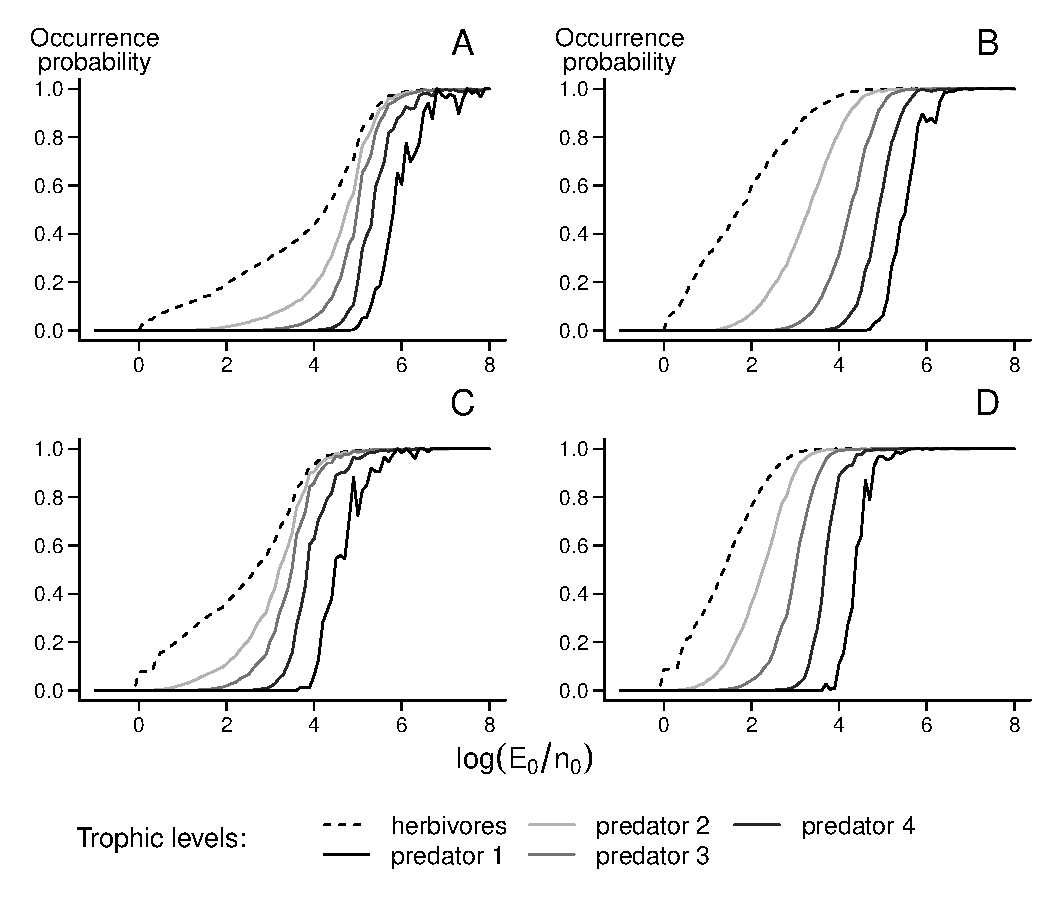
\includegraphics{fig/fig2.pdf}
\caption{\textbf{Species occurrence probability along an energy
gradient, grouped by trophic level}; herbivores, or by their shortest
path linking to a herbivore species. The top right letters indicates the
scenarios.\label{fig:etib2}}
\end{figure}

\begin{figure}[htbp]
\centering
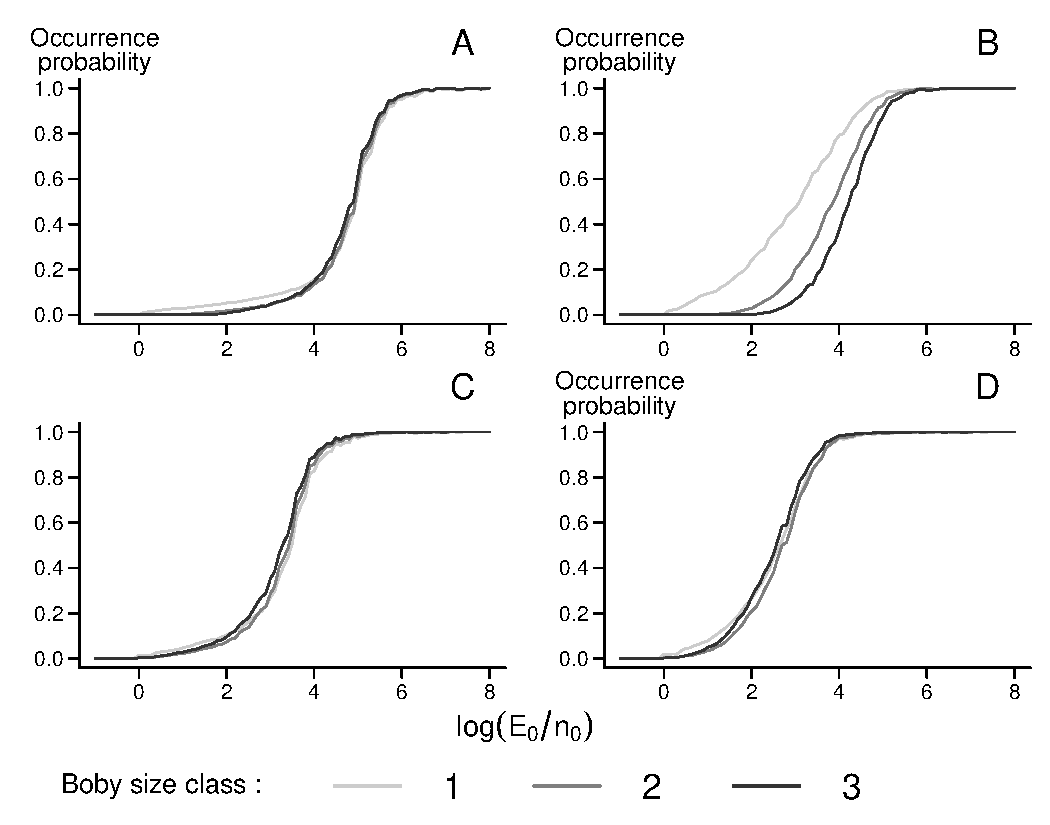
\includegraphics{fig/fig3.pdf}
\caption{\textbf{Species occurrence probability by energy gradient
grouped by body mass class}. The top right letters indicates the
scenarios.\label{fig:etib3}}
\end{figure}

\begin{figure}[htbp]
\centering
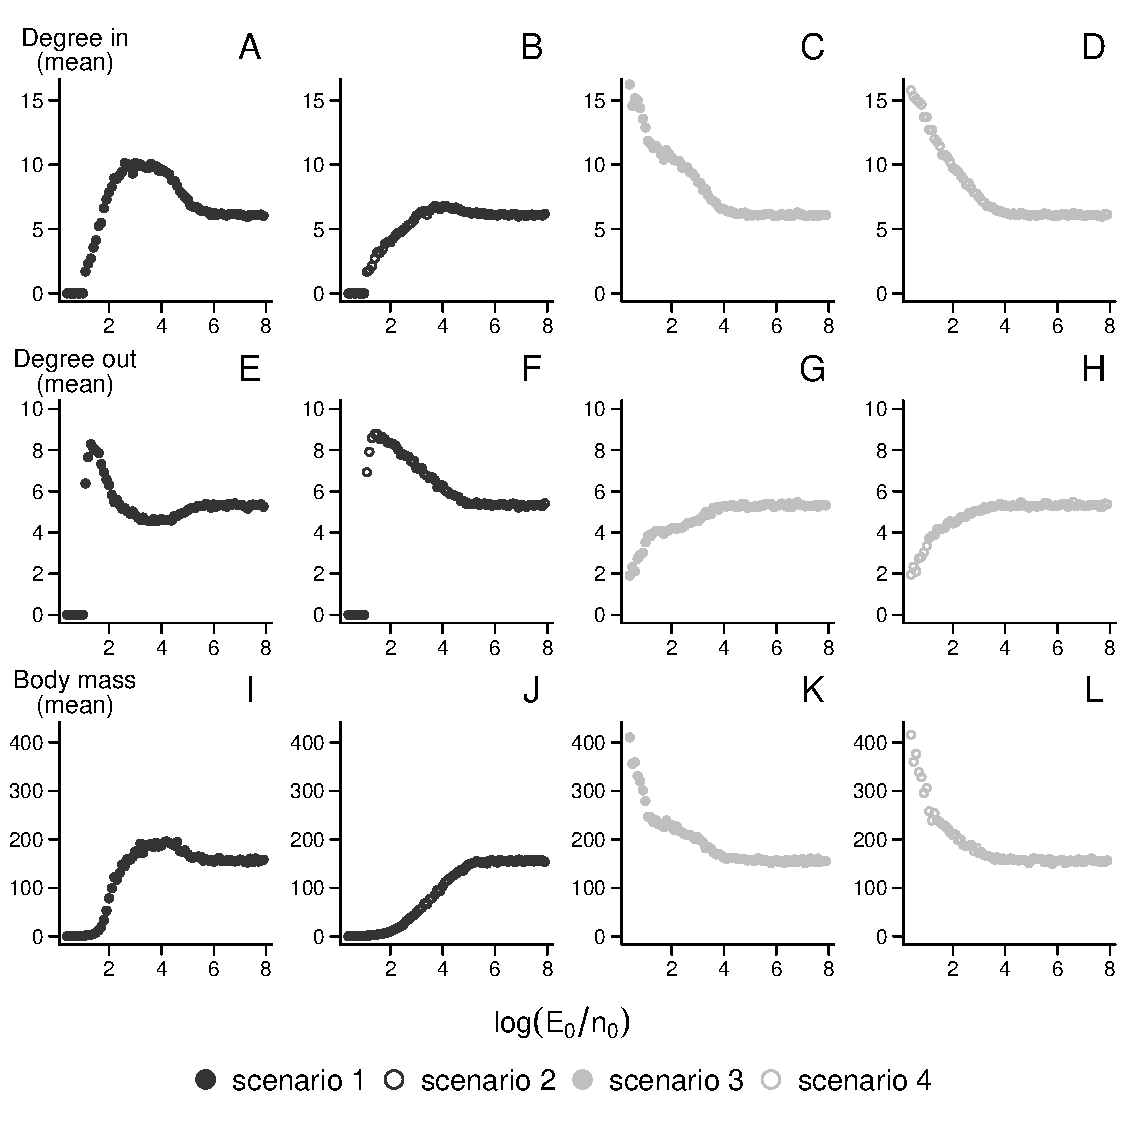
\includegraphics{fig/fig4.pdf}
\caption{\textbf{Average number of preys, predators, and mean body mass
of predator species on the island} in regards to the energy gradient for
four scenarios: (A) A,E,I, (B) B, F, J, (C) C, G, K, and (D) D, H,
L.\label{fig:etib4}}
\end{figure}
